\chapter{Terrain Data Exploration}
\label{chapter:TerrainDataExploration}

Chapter \ref{chapter:DrillOperator} discussed a novel terrain representation based on the drill operator, followed by a discussion in Chapter \ref{chapter:ErosionSimulation} of terrain data generation using an accurate and detailed hydraulic erosion simulation taking advantage of Smoothed Particle Hydrodynamics. A necessary next step toward fuller understanding of terrain data is the manipulation and exploration of said data. For this purpose, this thesis investigates a method of data interaction taking advantage of user interface design techniques. 

More specifically, this work investigates the use of laser pointers as collaborative user interface tools. The goal is the design and implementation of an interactive terrain surface data exploration tool used for the study of surface data, and a system that allows several users to collaboratively interact with the application simultaneously in an educational environment. 

\section{Laser Pointers as User Interface Tools}


\begin{figure}[t]
  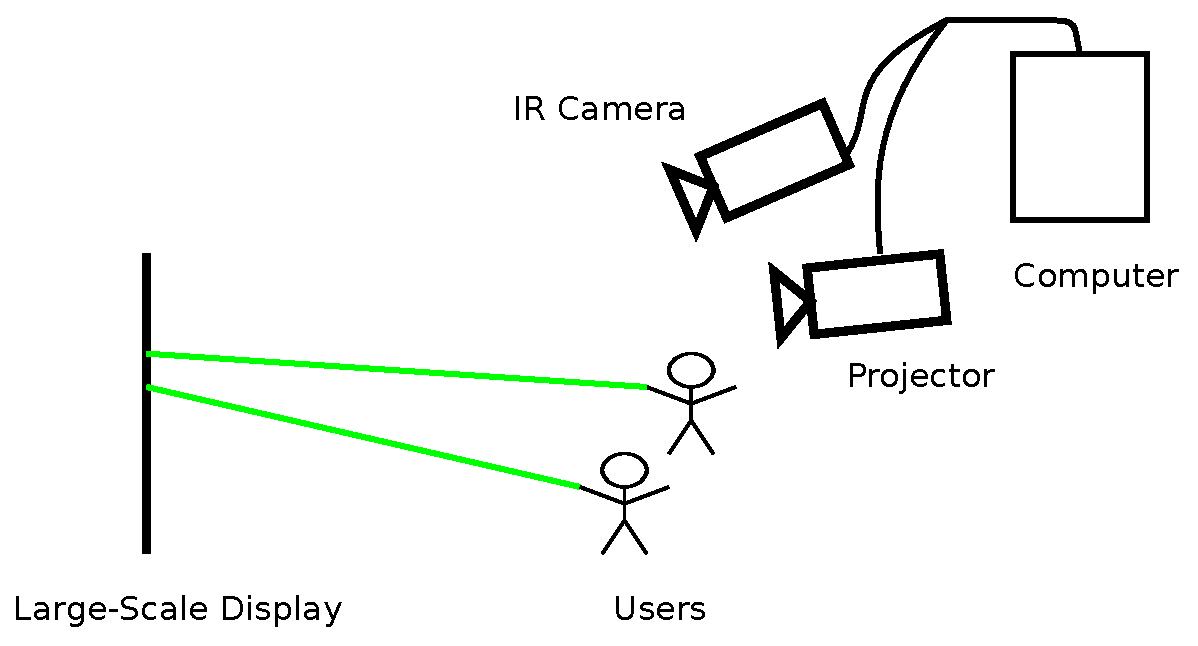
\includegraphics[width=1.0\textwidth]{images/Camera_Setup.eps}
  \caption[Schematic of laser interaction system setup]{\label{figure:LaserSetupSchematic}This is a schematic drawing of the system setup. In the system, multiple users train green lasers at a large scale projection surface, like a screen, onto which a projector is projecting images from an application. A camera with an infrared (IR) filter captures intensity images of IR light on the screen, and feeds the images to the computer controlling the system.}
\end{figure}



This work focuses on large scale interactive environments, such as those with a projector focused on a large screen. The setup of this system facilitates the use of laser pointers, and so they are a natural choice for interaction medium. 
% 
Multi-user, large-scale interfaces, in which individual users are uniquely identified, present a challenging and worthwhile design problem. In applications in which efficient interactivity between users is important, laser pointer devices are preferable to stationary pointer devices, such as mice \cite{Pavlovych:2008:ESC:1462027.1462035}. Setups in which each user controls his or her own mouse or other wired pointing device tend to be bulky and somewhat infeasible for larger numbers of users. In most cases, the challenge of identifying individual users is overcome by modifying laser pointers to be recognized and identified, an effective yet often-times costly and time-consuming solution. A schematic of the setup can be seen in Figure \ref{figure:LaserSetupSchematic}.



Single laser point detection is accomplished in two main ways:
brightness filtering and infrared filtering. Olsen and Nelson \cite{olsen2001} detect a
laser spot on a large display screen with a two pass
system. The first pass detects the brightest red spot
in the image, while the second (which only occurs if no obvious laser
spot is found) passes over the screen again, employing a convolution
filter, concentrating on the area where the last spot was detected. Oh
and Stuerzlinger \cite{Oh02laserpointers} allow for multiple laser points by applying a
threshold to the brightness field of the
image. The same technique is applied by Davis
and Chen \cite{Davis00lumipoint:multi-user} in their LumiPoint
system. However, depending on the
brightness of the laser spot with respect to the rest of the image can
create trouble, as it is context sensitive and simple thresholds may
confuse the laser points and very bright sections of the
image. Ahlborn, et al. \cite{Ahlborn:2005:PSL:1101616.1101637} present
a system using multiple camera views, in which the background image is
filtered out, leaving only laser points for detection. IR filtering is
employed by work by Qin, et al. \cite{Qin:2010:SLP:1842993.1843022},
Angelini, et al. \cite{angelini:multi-user}, and Cheng, et
al. \cite{Cheng:2003:DIL:857080.857088}.

\begin{figure}

\includegraphics[width=0.16\linewidth]{images/SpotPPMs/tagged_0_frame_492_point_FC_0.png}
\includegraphics[width=0.16\linewidth]{images/SpotPPMs/tagged_3_frame_728_point_FC_0.png}
\includegraphics[width=0.16\linewidth]{images/SpotPPMs/tagged_6_frame_977_point_FC_0.png}
\includegraphics[width=0.16\linewidth]{images/SpotPPMs/tagged_9_frame_1217_point_FC_0.png}
\includegraphics[width=0.16\linewidth]{images/SpotPPMs/tagged_12_frame_1484_point_FC_0.png}
\includegraphics[width=0.16\linewidth]{images/SpotPPMs/tagged_15_frame_1731_point_FC_0.png}%
\vspace{0.01in}

\includegraphics[width=0.16\linewidth]{images/SpotPPMs/tagged_1_frame_553_point_FC_0.png}
\includegraphics[width=0.16\linewidth]{images/SpotPPMs/tagged_4_frame_784_point_FC_0.png}
\includegraphics[width=0.16\linewidth]{images/SpotPPMs/tagged_7_frame_1038_point_FC_0.png}
\includegraphics[width=0.16\linewidth]{images/SpotPPMs/tagged_10_frame_1273_point_FC_0.png}
\includegraphics[width=0.16\linewidth]{images/SpotPPMs/tagged_13_frame_1536_point_FC_0.png}
\includegraphics[width=0.16\linewidth]{images/SpotPPMs/tagged_16_frame_1773_point_FC_0.png}%
\vspace{0.01in}

\includegraphics[width=0.16\linewidth]{images/SpotPPMs/tagged_2_frame_599_point_FC_0.png}
\includegraphics[width=0.16\linewidth]{images/SpotPPMs/tagged_5_frame_838_point_FC_0.png}
\includegraphics[width=0.16\linewidth]{images/SpotPPMs/tagged_8_frame_1085_point_FC_0.png}
\includegraphics[width=0.16\linewidth]{images/SpotPPMs/tagged_11_frame_1328_point_FC_0.png}
\includegraphics[width=0.16\linewidth]{images/SpotPPMs/tagged_14_frame_1594_point_FC_0.png}
\includegraphics[width=0.16\linewidth]{images/SpotPPMs/tagged_17_frame_1819_point_FC_0.png}

\vspace{-0.1in}
  \caption[False color renderings of laser IR spill]{\label{figure:laser_dots} 
False color renderings of the IR spill from 6 inexpensive green laser
pointers.  The pattern of this spill is relatively constant, allowing
us to track and identify the lasers over time.  The pattern of spill
from the laser varies most with distance of the laser to the screen.
The top row of images were collected with the laser 15 feet from the
screen, the middle row was 10 feet from the screen, and the bottom row was 5 feet from the screen.
}
\end{figure}

In addition to laser spotting, one challenge in multi-user laser
pointer systems is pointer identification. One method is to
dynamically change the number of lasers present in the system at any
given point in time, and to track an IDed laser spot across frames
with predictive measures, such as the Kalman
filter~\cite{Oh02laserpointers,Davis00lumipoint:multi-user,Cheng:2003:DIL:857080.857088}.
Another method involves the use of time division multiplexing, or the
application of a laser blinking pattern, to identify a particular
laser. Given \emph{n} lasers, a system can force exactly one of the
lasers off each frame. With cameras with high frame rates, this
produces an unnoticeable effect with regard to the temporal coherence
of the laser spot on the screen, but the system can identify the laser
by its blinking pattern. These systems, however, are limited in the number of lasers
that can be included in the system, based on the frame rate of the camera.
This method is employed by Vogt, et
al.~\cite{Vogt:2004:ECG:1009379.1009663,Vogt03trackingmultiple}, as
well as Pavlovych and Stuerzlinger~\cite{Pavlovych04laserpointers}.

Laser point detection, both single- and multi-user, has a variety of
applications, most of which revolve around user collaboration and
interaction. Francisco de la O Chavez et al. \cite{delaOChavez:2008:INL:1387269.1387276} present a system
whereby users can operate the electronic devices and appliances in
their homes with a laser pointer. The system uses a
single camera, and the user sets up ``active zones'', or groups of
pixels in the camera view around each appliance. When a laser spot is
detected in the active zone, the appliance is activated. Qin et al. \cite{Qin:2010:SLP:1842993.1843022}
present a system in which a special laser pointer is used to project
several beams, and the orientation of the beams indicates the angle of
rotation along the beam axis of the laser, thus allowing for gestures
and object manipulation that involves rotation. Bi et al. \cite{BiUpen} present the uPen, a
laser pointer outfitted with right- and left-click buttons, designed
to mimic computer mouse functionality.
Shizuki et al. \cite{Shizuki:2006:LPI:1133265.1133284} present a series of 
gestures used with a laser pointer, and a series of applications using them.
The gestures are edge-crossing gestures, and the applications presented include 
a presentation application using gestures to move slides forward, and a picture 
viewing application where gestures manipulate the images.

To my knowledge, no work has been published regarding the
identification of off-the-shelf laser pointers in multi-user
applications. Also, the domain of applications that have been explored
for multi-user laser pointer interaction is rather small, either due
to lack of need or due to the necessity of engineering laser pointers
to make the interfaces effective.




\section{Laser Personalities}
\label{section:LaserPersonalities}



\subsection{Laser Identification System Details}
\label{section:systemdetails}

To detect the current position of each laser pointer dot, a
1280 x 960 pixel monochrome, 33fps video camera is used.  An infrared (IR)
pass filter in front of the camera blocks all visible light (from the
projector), so the bright points of IR light
from the laser can be robustly detected. Green laser pointers are used because the
green light is produced indirectly from an infrared laser diode, and
some of the infrared light remains for our detection.  Most
inexpensive green lasers do not include an IR filter to block this
light.

The system begins with a simple
calibration step to determine the pixel to
pixel correspondence between the camera and the 1920 x 1080 projector
and 
%18' tall screen.  
projection surface, and to collect intensity data on all lasers in the system. The system has been tested on screens as tall as 18'.
This step consists of shining one or more lasers at a 3x4 grid of
calibration points.  The first geometric calibration
% DOES IT? I AM CONFUSED
allows the identification of
multiple lasers simultaneously pointed at the screen.  For non-erratic
laser motions, these points can be easily tracked over time to allow
users to perform actions within an application.
% , for example {\em
%   moving} pieces around in a jigsaw puzzle (Figure~\ref{figure:puzzle}) or
% {\em circling} nodes in a graph visualization (Figure~\ref{figure:graphVisualization}).

When tracking multiple lasers simultaneously, the Kuhn-Munkres,
a.k.a. {\em Hungarian
  Algorithm}~\cite{kuhn,munkres,munkres_implementation} is used to match the
lasers from frame to frame.  This method produces a pairing that
efficiently minimizes the sum of the distances between the positions
of each laser between the two frames.  Also considered for this purpose was a
Kalman filter~\cite{Kalman} to track smoothly moving laser dots, but
early experiments indicated this was complicated to tune for the
accelerations of the laser dots at corners or tight turns and
ultimately not necessary.

\subsection{Laser Spot Processing}

\begin{figure}[t]
  \centering
  \includegraphics[width=0.6\textwidth]{images/LaserHistogramExample_crop.png}
  \caption[Diagram of histogram to calculate laser histogram]{\label{figure:LaserHistogram} This figure presents an example of how to build the histogram of intensity values. For each pixel-sized ring, the average intensity is calculated. This value is stored in the corresponding histogram.}
\end{figure}
% 
% \begin{figure}[t]
%   \centering
%   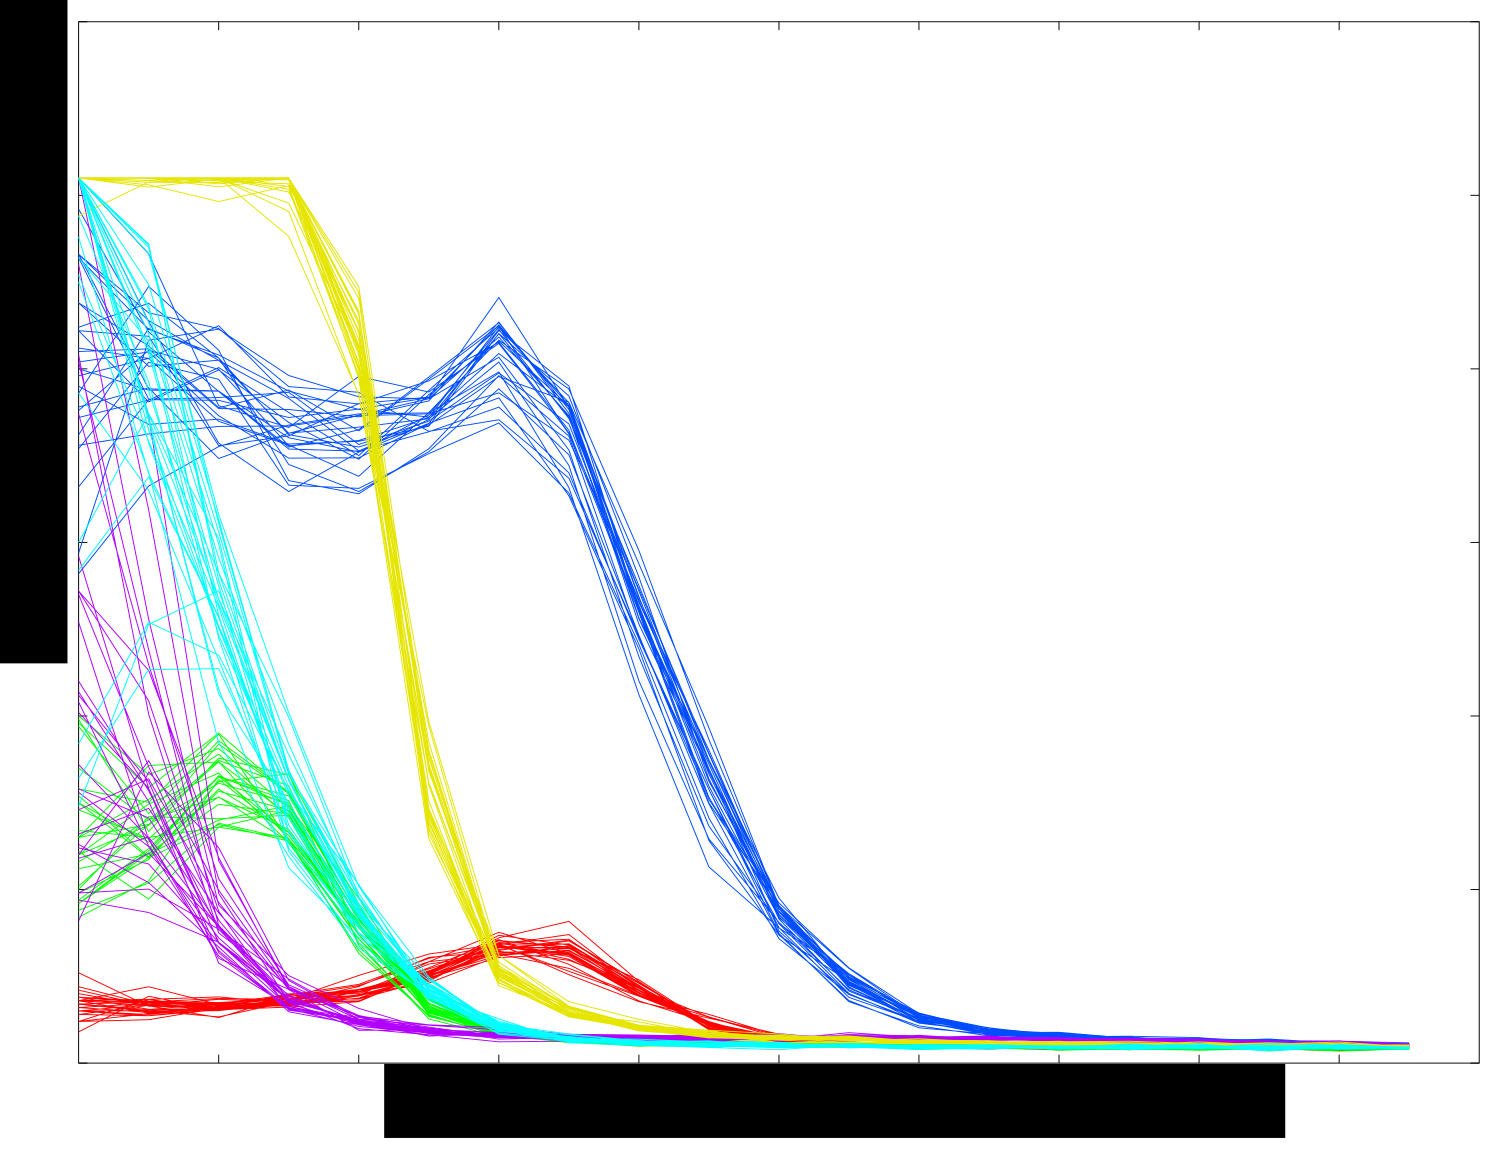
\includegraphics[width=1.0\textwidth]{images/AllLaserPersonalities_OneSpot.png}
%   \caption[Laser personality training data]{\label{figure:PersonalityTrainingData}}
% \end{figure}

In addition to the centroid of the laser spot the
intensity and size of the detected blob is extracted
%variation in from these sample points of infrared light in order to
to calibrate laser intensity data for identification.  Inexpensive
lasers exhibit a range of brightness and focus, as shown in
Figure \ref{figure:laser_dots} and this signature is fairly consistent
for each device (once the laser has warmed up for about 15 seconds,
and as long as the batteries are reasonably fresh). This
signature is called the laser's \textit{personality}.
% We examine the blob of light at each detected laser point and fit a
% two parameter (radius \& brightness) Gaussian to the data.  
During the calibration phase, several frames' worth of this
intensity data are captured at each of the calibration points for each laser. The blob of light 
is examined and a radial histogram of the intensity values of the blob is calculated. An image of this histogram can be seen in Figure \ref{figure:LaserHistogram}. 
In practice, 20 bins (representing a
radius of 20 pixels) is sufficient to capture the uniqueness of a
laser spot's shape.  This intensity histogram acts as the laser's
personality.
% We perform
% an intensity calibration for each laser, again by pointing the laser
% at each calibration grid point.  
Note that the calibration can be performed simultaneously for many
lasers (with 1 person per laser), and takes less than a minute.  The
laser personality intensity calibration could also be performed
passively and continuously, which is explored in future work.
Sample laser personality data is presented in
Figure~\ref{figure:six_laser_personalities}.


\begin{figure}
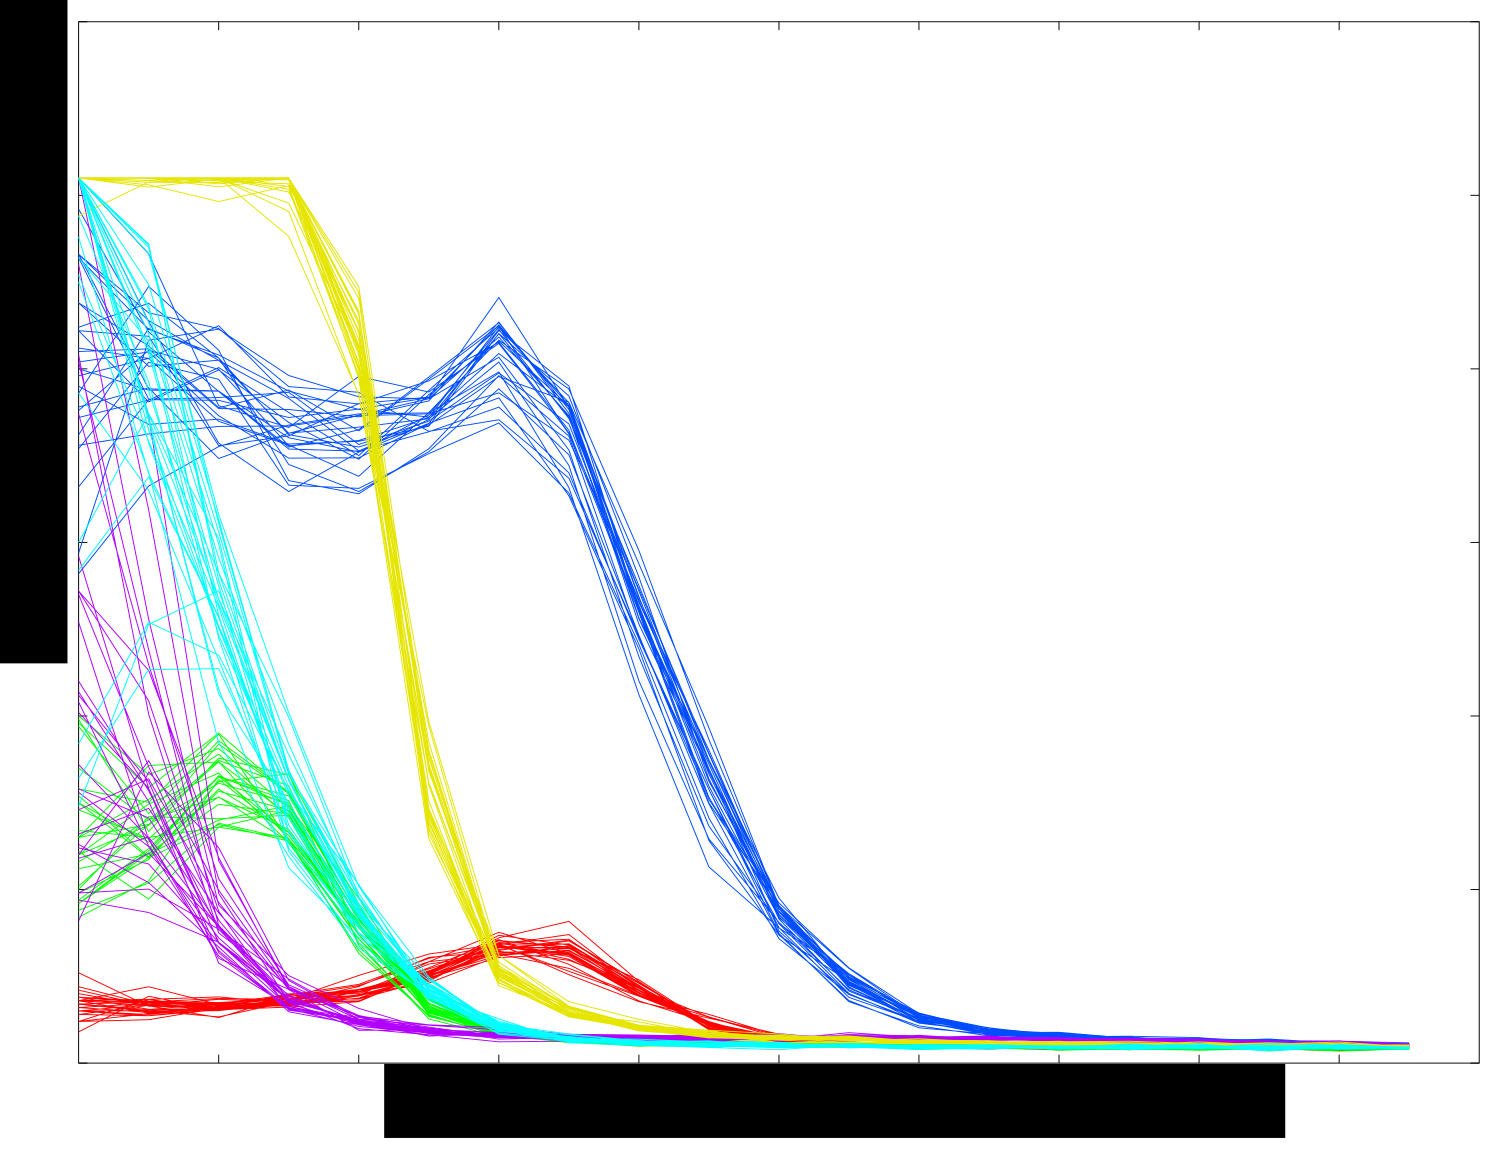
\includegraphics[width=0.99\linewidth]{images/AllLaserPersonalities_OneSpot.png}

\vspace{-0.1in}
\caption[Laser personality training data]{\label{figure:six_laser_personalities} This figure shows 30
  personality measurements for each of 6 lasers from a single
  calibration screen location. A single data point (a laser
  personality measurement) is represented by a radial histogram of
  intensities arranged by distance from the centroid of the laser
  spot, and each line represents one such data point. Each laser is
  represented by a different color. The intensity measurements range
  from 0 to 255 (y-axis), and the distances from the centroid of the
  laser spot range from 0 to 20 (x-axis). As an example, the blue
  laser's spot reaches its peak intense approximately 6 pixels from
  its center.
}
\end{figure}


\subsection{Identifying Laser Spots: Matching Personalities}

Once calibration is complete, the system is able to match any laser
spot on the projection surface with one of the calibrated lasers.
When a laser spot is detected, its personality is calculated, and
matched with that of one of the known lasers.

For efficiency, the system utilizes two passes to process the camera image.  In
a first coarse pass, every $n$th pixel in the camera image is examined
and all pixels greater than a pre-set intensity threshold continue to
the second pass.  In the second pass, a generous window around each
seed pixel is examined.  All nearby pixels above the
threshold are collected and the largest connected component is extracted.  
The centroid of this component is set as the laser spot position.  The system then computes
the histogram of pixel intensities shown in
Figure \ref{figure:six_laser_personalities}.  The final task is to
match the detected histogram to the library of known lasers, collected during calibration.  
This matching is accomplished by calculating the sum of squared differences between
the detected histogram and the histogram of each each known laser, and the laser ID assigned to the new histogram is the ID of the laser whose personality with the minimum sum.

It is important to note that the apparent laser intensity varies
spatially for each laser due to a number of additional variables,
including: distance from laser to screen, distance from screen to
camera, and camera vignetting.  
% They can easily normalize for thesevariations.
Normalization is accomplished by 
averaging all of the intensity data for all of the lasers collected
at each of the calibration grid points, and then normalizing the
input by dividing it by the spatial average normalizes the data for camera position.
Barycentric coordinates and interpolation normalizes the laser points 
between calibration grid locations.
Camera position normalization is especially crucial when the camera is placed
at an extreme angle to the screen, and thus experiences significant
perspective distortion.

% First, we normalize for the camera position by averaging
% all of the intensity data for all of the lasers collected at each of
% the calibration grid points, and normalize the input by dividing it by
% the spatial average.  We use barycentric coordinates and interpolation
% to normalize laser points between calibration grid locations.  

Just as the camera position relative to the screen is important, the
laser spots also exhibit perspective distortion when they are used at
extreme angle to the screen.  This distortion can similarly be normalized for, assuming that the intensity calibration data for each
laser is collected from a position near that laser's use location.

% \subsection{Temporal Coherence and Simultaneous Use}

% For the tests presented in this paper and companion video we do not
% leverage temporal coherence in our detection.  Because the camera
% image and laser output contain some noise, the quality of the
% personality measurements and identification would benefit from
% averaging the output of multiple frames known to be the same laser
% from the tracking algorithm in Section~\ref{section:systemdetails}.

When multiple lasers are simultaneously detected on the screen, the system can
leverage this information to disambiguate lasers with somewhat similar
histogram personalities.  The system employs the Kuhn-Munkres algorithm to
assign unique labels to all detected points; that is, no two lasers
will be assigned the same ID, even if they both select the same ID as
their first choice.



\section{Accuracy Testing}
\label{section:TestResults}

%PLACEHOLDERS!
\begin{figure}
  \centering
  \includegraphics[width=0.99\linewidth]{images/room_diagram_annotated.png}
  \caption[A diagram of the laser personality testing space]{\label{figure:laser_testing_room_diagram} A diagram of the testing space. 'X's are marked in arcs at intervals of 5' from the center of the projection surface, separated by $22.5\,^{\circ}$ arcs. Five locations (A through E) are marked on the diagram for reference. }
\end{figure}


\begin{center}
\begin{table*} [t]
\centering
\caption[Laser personality accuracy testing data]{\label{table:AccuracyTestingResults}Results from accuracy
  tests. Five tests were performed in all (Single Position Test = SP, Arc Movement Test = AM, Line Movement Test = LM, Walking Path Test = WP, All Lasers Test = AL), and for each test and for
  each laser two percentages are reported: the percentage of frames in
  which it was correctly identified as its primary ID (left column), and the
  percentage of frames in which it was identified as either the primary or secondary
  ID (right column). The minimum number of frames collected for each test is reported
  along the bottom row. 
  }
\begin{small}
\begin{tabular}{ | c | r | r | r | r | r | r | r | r | r | r | }
 \hline
 \textbf{} & \multicolumn{2}{|c|}{\textbf{SP}} & \multicolumn{2}{|c|}{\textbf{AM}} & \multicolumn{2}{|c|}{\textbf{LM}} & \multicolumn{2}{|c|}{\textbf{WP}} & \multicolumn{2}{|c|}{\textbf{AL}} \\
 \hline
  1 & 100.00 & 100.00& 96.54 & 98.27 & 53.88 & 74.14 & 51.13 & 68.49 & 99.79 & 100.00 \\
  2 & 100.00 & 100.00 & 100.00 & 100.00 & 90.43 & 95.21 & 78.65 & 86.25 & 99.07 & 100.00 \\
  3 & 95.85 & 100.00 & 70.96 & 73.48 & 35.14 & 48.65 & 60.50 & 96.10 & 83.49 & 98.75 \\
  4 & 92.79 & 100.00 & 77.40 & 100.00 & 80.41 & 100.00 & 83.02 & 100.00 & 99.61 & 99.78 \\
  5 & 99.67 & 99.67 & 100.00 & 100.00 & 57.99 & 92.57 & 82.95 & 94.26 & 99.80 & 99.92 \\
  6 & 90.33 & 96.03 & 93.89 & 95.91 & 72.56 & 79.70 & 91.81 & 94.86 & 84.08 & 99.90 \\
  \hline
  \textbf{} & \multicolumn{2}{|c|}{521} & \multicolumn{2}{|c|}{347} & \multicolumn{2}{|c|}{230} & \multicolumn{2}{|c|}{645} & \multicolumn{2}{|c|}{968} \\
 \hline  
\end{tabular}
\end{small}
\end{table*}
\end{center}

Several tests were performed to judge various notions of accuracy of the
\emph{laser personality} system. The tests were performed using six
lasers (given IDs 1-6) in the 19' x 23' space shown in Figure
\ref{figure:laser_testing_room_diagram}. The space was divided into a
series of testing locations, marked with an 'X' in the diagram, at
discretized $22.5\,^{\circ}$ arcs with radii of 5', 10', and 15' from
the center of the projection surface.

Two sets of calibration data were collected. For the first calibration
(referred to from now on as calibration $C1$), all six lasers were
calibrated from the 15' mark along the line perpendicular to the
projection surface (point A in Figure
\ref{figure:laser_testing_room_diagram}). For the second set of data
(calibration $C2$), all six lasers were calibrated simultaneously from
different points along the 10' arc (point B resides on this arc). The
accuracy of a laser was defined as the percentage of frames in which
the laser was identified correctly out of all detection frames. These
results are presented in Table \ref{table:AccuracyTestingResults}.

%During testing, a concerted effort was made to maintain a consistent
%number of data collection frames within each test, and so 
The minimum number of frames considered for each test is reported in
Table \ref{table:AccuracyTestingResults} along the bottom row. Five
accuracy tests were run in total, with users stationary, walking in an
arc, walking along a straight line, walking along a path, and using
all lasers simultaneously. For the tests, we count the number of times
the laser is correctly identified as the primary choice, and the number of times the correct
laser is the secondary choice (the laser intensity histogram with the
next smallest sum of squared differences). These two values comprise
the two columns in Table \ref{table:AccuracyTestingResults} for each
test, with the primary ID on the left and the secondary on the right.

\subsection{Description of Tests}

The first four tests all used calibration data $C1$, while the final
test used calibration data $C2$.

\textbf{Single Position Test} The purpose of this test was to judge how
well lasers could be matched to the calibrated data. Data was recorded
from the position at which the calibration $C1$ was collected,
position A, and the tester did not move from that location. Each laser
was shone on the screen for at least 521 frames (roughly 17.75
seconds), making sure to point at both the middle and each of the four
corners of the screen. Each laser was correctly identified in at least
90\% of the frames taken, and each laser was either identified
correctly or as the secondary laser at least 96\% of the time.

\textbf{Arc Movement Test} The purpose of this test was to judge how
much side-to-side movement affected the overall accuracy of the
identification system, because the shape of the laser spot is skewed
when seen from an angle, changing the laser's personality. Data was
recorded while users walked along the 10' arc of data collection
points, passing right-to-left through point B. The laser was kept as
close to the center of the screen as possible to avoid affecting the
laser spot in additional ways. Each of these tests lasted at least 347
frames (roughly 11.5 seconds). Four of the lasers performed well (with
at least 93\% accuracy), while lasers 3 and 4 maintained 70\%
accuracy. Each laser was identified as either its first or second
choice laser ID in at least 93\% of the frames, except laser 3.

\textbf{Line Movement Test} The purpose of this test was to
judge how much distance from the screen affected the overall accuracy
of the system. Changing the distance to the projection surface changes
the radius and intensity of the laser spot, and thus affects the
histogram of the laser's personality. For this test, the user stood as
far from the screen as possible (approximately 20') and walked forward
to the 5' mark, perpendicular to the screen. The laser was once again
kept as close as possible to the center of the screen. Each of these
tests lasted at least 230 frames (roughly 7 seconds). The results for
this test were significantly poorer than other tests, as three of them
scored below 60\% (laser 3 scored below 40\%).
% This was the only test
%in which one of the lasers was more often identified as its secondary
%ID (laser 3) than its primary.

\textbf{Walking Path Test} The purpose of this test was to provide an
overall averaging of the previous two tests, and to mimic movement
expected by users in real-world environments. The path taken followed
the letters marking room positions in Figure
\ref{figure:laser_testing_room_diagram} from position A to B, C, D, E,
and back to A. The laser was again kept as close as possible to the
center of the screen. Each of the tests lasted at least 645 frames
(roughly 19.5 seconds). In general, the lasers performed as expected,
an average somewhere between the arc and the straight line tests. Only
laser 1 fell below 60\% accuracy, while none of the other lasers beside laser 1 had more
than 15\% failure to be the first or second choice histogram
personality.

\textbf{All Lasers Simultaneous Test} The purpose of the final test
was the assess how accurately the laser identification system
performed when several lasers were on the screen at once. In this
test, users stood at each of 6 marks along the 10' arc (the positions
from which calibration $C2$ data was collected) and all shone lasers
at the screen simultaneously. The laser spots followed a path that
touched all four corners as well as the middle of the projection
surface.  Two lasers, 3 and 6, were confused with one another in
approximately 15\% of the frames, but each of the other 4 lasers were
at least 99\% accurate.

\subsection{Results and Discussion of Laser Accuracy Tests}

Overall, the laser identification system is effective and useful for a
variety of applications. It is overwhelmingly effective when lasers
remain in the general area from which their calibration data is
collected while the system is in use. It is rare that a laser is
mislabeled in this instance. Many multi-user applications do not
require users move around the room while the system is in use, such as
education applications in a classroom environment, or games played
collectively by an audience. However, when moving from place to place,
the shape of the laser spot can change dramatically, and so the
personality can as well. As is to be expected, this is most extreme
when moving a different distance from the projection surface, as the
spot's intensity signature changes and its radius grows and shrinks
dramatically, making histogram comparison considerably more difficult.

These tests bring to light two significant shortcomings of the
identification system. The first is that position is important when
comparing a laser spot to a given set of laser personalities,
especially distance from the projection surface. The farther one moves
from the spot of calibration, the less accurate the laser
identification becomes. However, even in tests where the distance to
the screen changed, most of the lasers performed well. The system's
second shortcoming is that a laser's personality changes over the time
of its use. Battery-powered laser pointers change the range of their
output intensities as their batteries drain and the lasers themselves
warm up. Therefore, it is often the case that, over the course of its
use, a laser's personality will shift away from the data collected
during the calibration phase. 

Both of these shortcomings can be
addressed by the idea of continuous calibration, discussed in Section \ref{section:SummaryAndFutureWorkDataExploration}.


\section{Terrain Data Exploration Application}

\begin{figure}
  \begin{center}
  \begin{minipage}{0.79\linewidth}
     %a)
    \includegraphics[width=0.49\linewidth]{images/terrain1.jpg}
     %b) 
    \includegraphics[width=0.49\linewidth]{images/terrain2.jpg}
  \end{minipage}  \\
  \begin{minipage}{0.79\linewidth}
    % c) 
    \includegraphics[width=0.99\linewidth]{images/terrain3.jpg}     
  \end{minipage}  \\
  \begin{minipage}{0.79\linewidth}
    %d) 
    \includegraphics[width=0.49\linewidth]{images/terrain4.jpg}
    %e) 
    \includegraphics[width=0.49\linewidth]{images/terrain5.jpg}
  \end{minipage}  
  \end{center}
  \caption[Visualization of the terrain hydrography exploration tool]{\label{figure:hydrographyVisualization} A visualization of the terrain hydrography exploration tool, which takes in as input a height field and visualizes it. Notice the channel highlighted by the top left image, and water flow down the channel in the top right and middle images. While user \#1 adds rain to the terrain, user \#3 begins to raise the land, damming the channel (lower left image), until the hydrography information has been updated and the water must flow around the newly formed dam (bottom right image). }
\end{figure}


Data manipulation in a multi-user environment can be a powerful teaching tool. To this end, a visualization tool for terrain hydrography analysis, seen in Figure \ref{figure:hydrographyVisualization}, has been developed.
The goal of the application is to allow for the exploration of terrain hydrography data by multiple users through a laser pointer interface. The application consists of a data view and a graphical user interface side-by-side, in which modes are selected in the GUI through dwell-selection. In addition to selection of modes, the laser pointers are also used to interact directly with the 3D terrain data and camera view.
%, depending on the current mode of the program.

The application takes as input a height field,
% (a scalar field of height values arranged on a regular grid), 
which represents the terrain to be visualized. The terrain is drawn in the data view section of the display, color coded according to scalar value (height, in this case) and normalized to fit the range of maximum to minimum values of the data. The user selects a mode using buttons on the right side of the screen. These modes include camera position modes (Rotate, Translate, Zoom), visualization modes (Watershed and Channel Network), and interaction modes (Add Rain, Lower Land, Raise Land). Because each user can have any mode active at any given point in time, multiple updates to the data and visualization can occur simultaneously. When a button is selected, the application identifies the laser pointer that made the selection and associates it with the corresponding mode. For example, if laser \#3 selects the Rotate mode, a small ``3'' appears on the Rotate button and laser \#3 can now rotate the camera through a click-and-drag motion in the data view window.

Upon read in of the data (and every time it is altered by one of the
interaction modes), the hydrography information of the terrain is
determined using 
% both a variation of the least-cost flow routing method by Metz et al. \cite{hess-15-667-2011}, and the flow accumulation method presented by O'Callaghan and Mark \cite{O'Callaghan1984323}. 
the method introduced in Chapter \ref{chapter:DrillOperator}.
The least-cost flow routing is fast
enough in its implementation to allow the hydrography information to
be updated in interactive time (approximately 15 to 20 FPS). This is
important, as interaction with the data and the camera view should not
impede exploration of the data by other users.

The camera position modes allow users to rotate, translate, and zoom the camera, changing the view of the data, as described above. Watershed and Channel Network modes both visualize hydrography information on the terrain surface. While in watershed mode, a laser point detected on the surface of the data highlights the watershed of the corresponding space on the data. When Channel Network mode is active, the channels of the terrain are visualized. 
%These two modes can be seen in figure \ref{figure:WatershedAndChannelNetwork}.
Finally, interaction modes allow the users to manipulate the
data. Raise and Lower Terrain modes allow the user to raise and lower
the surface data by selecting a space on the data. The data is
manipulated according to a radial Gaussian filter, centered at the
space selected by the laser. This, in essence, grows hills and
craters. When Add Rain mode is selected, the user can select a space
on the terrain, and rain drops fall onto the surface in a radial
pattern centered at the selected space. The rain then flows, according
to the internal hydrography information, down hill and off the edge of
the terrain. These modes are demonstrated in
Figure~\ref{figure:hydrographyVisualization}.

The multi-user nature of the application allows some users to be manipulating the data itself, while others explore the repercussions of this manipulation (by creating rain drops and watching where they flow and highlighting various watersheds along the path of the flowing water), all while others manipulate the camera, perhaps following the path of the water as it flows between mountains and off the edge of the terrain. Users have commented informally that the ability to manipulate the surface data while watching rainwater flow across the terrain was particularly useful, as it demonstrated how much hydrography can change with slight alterations to the terrain.

\section{Summary and Future Work of Terrain Data Exploration}
\label{section:SummaryAndFutureWorkDataExploration}

This chapter has presented a system for interactive group problem solving and data exploration using inexpensive, off-the-shelf laser pointers as user interaction media. The system uses the IR light leaking from the lasers as a method for measuring the laser's personality,
% or IR splotch, 
allowing for individual laser identification. The system was used to develop an interactive exploration tool for terrain data, in which several users can simultaneously explore the terrain, cause rain to fall on the terrain (thus demonstrating the terrain's hydrography), and alter the surface. All updates are at interactive rates, so it the terrain is changed while water flows over it, the water directions may well change. 

The key to the expanded use of this system is that there is no additional engineering required. The lasers users are all inexpensive, and can be used as purchased without additional modifications. 
The camera 
% is inexpensive, and 
only requires an IR filter. 
% Several additional applications have been designed for this system, from puzzle solving, to gaming (Pong, for instance), to group problem solving. 
The system is robust and mobile, and as such can be installed in many different environments, including classrooms for use in collaborative learning exercises. 
% The possibilities of this system are nearly endless. 


% Future work for the system is described in Section \ref{section:FutureWork}.

% \section{Future Work for Terrain Data Exploration}

The laser personality system will be improved as future work.
While the system works well when users do not change how far they are from the project surface (sufficient for many applications), there are times when this is not enough. One clear extension to this work is the introduction of continuous calibration. First, the special calibration step will be omitted, and instead initial calibration will be generated from early incidental usage, and the system will continue to dynamically update a laser's data as it is used. As new data is added to the system, older data will be replaced, and so the calibration data will change as the lasers' personalities do. This continuous update of the calibration data will allow for less confusion between laser spots as the laser points warm up and change from continuous usage. 

The applications will also be improved. One such improvement would be a move to a multiple-screen multiple-camera format. Laser strokes will need to be ``passed off'' accurately from one camera's view to the other's, and each viewing system will need to be calibrated independently (unless dynamic calibration is implemented). The applications will be improved to more fully take advantage of identifiable laser points. For instance, there will be a user feedback system for a puzzle-solving application, in which users who are contributing to solving the puzzle accurately will be rewarded while those who are destructive may face a penalty to their piece-moving privileges. This would mimic real-world collaborative reward systems.

